% Generated by AP Math GOLD PILOT deterministic Python generator.
% input id: 03_circle_center_radius
\documentclass{article}
\usepackage[margin=1cm]{geometry}
\def\pgfsysdriver{pgfsys-dvisvgm.def}
\usepackage{amssymb}
\usepackage{pgfplots}
\pgfplotsset{compat=1.18}
\pagestyle{empty}
\begin{document}
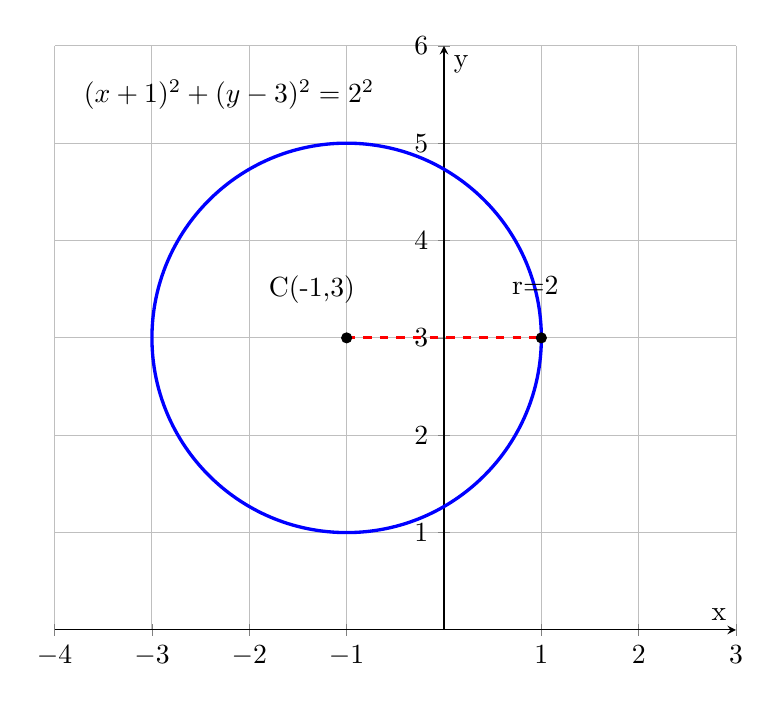
\begin{tikzpicture}
\begin{axis}[width=13cm,height=9cm,axis equal image,axis lines=middle,grid=major,xmin=-4,xmax=3,ymin=0,ymax=6,xlabel={x},ylabel={y},clip=true]
\draw[blue, solid, line width=1.2pt] (axis cs:-1,3) circle [radius=2];
\draw[red, dashed, line width=1pt] (axis cs:-1,3) -- (axis cs:1,3);
\addplot[only marks,mark=*,mark size=1.8pt,black] coordinates {(-1,3)};
\addplot[only marks,mark=*,mark size=1.8pt,black] coordinates {(1,3)};
\node[anchor=south west] at (axis cs:-3.8,5.25) {$(x+1)^2+(y-3)^2=2^2$};
\node[anchor=south west] at (axis cs:-1.9,3.25) {C(-1,3)};
\node[anchor=south west] at (axis cs:0.6,3.35) {r=2};
\end{axis}
\end{tikzpicture}
\end{document}
